\documentclass{article}
\usepackage[brazil]{babel}
\usepackage[utf8]{inputenc}
\usepackage{url}
\usepackage{multicol}
\usepackage[bottom=2cm,top=2cm,left=1.8cm,right=1.8cm]{geometry}
\usepackage{graphicx}
\usepackage{float}
\usepackage{caption}
\usepackage[dvipsnames]{xcolor}
\usepackage{tikz}
\usepackage{amssymb}
\usepackage{setspace}
\usepackage{indentfirst}
\usepackage{mathtools}
\usepackage{amsmath}
\usepackage{subfigure}

\title{Lista 3\\
\large Sistemas Baseados em Conhecimento: \texttt{[MAC0444]}}
\author{Julia Leite - \texttt{11221797}}

\begin{document}
    
\maketitle

\textbf{1)} \textit{João é cardiologista. Sua irmã, Marta, está desempregada. O pai deles dois, Pedro, 
é casado com Olívia, uma geriatra. Pedro é arqueologista e tem dois filhos no total.}\\

\textbf{a)} $Human \sqcap \neg Famale \sqcap (\exists married.Doctor) \sqcap (\forall hasChild.(Doctor \cap Professor))$

Onde:

\begin{itemize}
    \item [-] \textit{Human}: é humano(a)
    \item [-] \textit{Female}: é do sexo feminino
    \item [-] \textit{Doctor}: é médico(a)
    \item [-] \textit{Professor}: é professor(a)
    \item [-] \textit{hasChild(x, y)}: x tem y como filho(a)
    \item [-] \textit{married(x, y):} x é casado(a) com y
    %\item [*] $\cap$: conjunção 
\end{itemize}

O conceito acima diz respeito a um humano que não é mulher, que é casado com ao menos um médico e cujos filhos são médicos ou professores.

\textbf{b)} \textit{Considerando apenas as quatro pessoas mencionadas, João, Marta, Pedro
e Olívia, podemos afirmar que algum deles pertence a esse conceito? Justifique.}\\

Não. As moças mencionadas não cumprem os requisitos de não ser do sexo feminino. Já João não é
casado com um(a) médico(a) e Pedro tem uma filha que, no momento, não é médica nem professora.\\

\textbf{c)} \textit{Se uma das 4 pessoas acima não existisse, sua resposta mudaria? Como e por quê?}\\

Se Marta não existisse, Pedro pertenceria a esse conceito já que, os filhos (se houverem) precisam ser médicos ou 
professores, mas não é obrigatório ter um filho de cada categoria.\\

\textbf{2)} T-Box $\tau$:

\begin{enumerate}
    \item  $Mulher \sqsubseteq Pessoa$
    \item  $Homem \sqsubseteq Pessoa$
    \item  $Homem \sqsubseteq \neg Mulher$
    \item  $Mulher \sqsubseteq \neg Homem$
\end{enumerate}

Vamos verificar se o axioma abaixo é consequência lógica de $\tau$, 
supondo uma interpretação $I$ arbitrária de $\tau$

$$Pessoa \sqcap \neg Homem \equiv Mulher$$

\newpage

Vamos provar a equivalência em duas etapas:

\textbf{I.} $Mulher \sqsubseteq Pessoa \sqcap \neg Homem$

Então, seja um elemento $x$ tal que $Mulher(x)$

Utilizando 1, sabemos $Pessoa(x)$
e com 4, temos $\neg Homem(x)$mandei naquele go de comp movel um vídeo de como faz, então:

$$Pessoa(x) \sqcap \neg Homem(x)$$

\textbf{II.} $Pessoa \sqcap \neg Homem  \sqsubseteq Mulher$

Seja $x$ tal que $Pessoa(x)$, $\neg Homem(x)$ e $\neg Mulher(x)$

Podemos observar que $x$ satisfaz nossa base de conhecimento, contudo, 
torna a afirmação \textbf{II} falsa.

Logo, o axioma não é consequência lógica de $\tau$

% Vamos provar essa afirmação mostrando que não existe um elemento $x$ 
% no domínio tal que 
% $Pessoa(x) \sqcap \neg Homem(x) \sqcap \neg Mulher(x)$

% $$Pessoa(x)$$
% $$\neg Homem(x)$$
% $$\neg Mulher(x)$$

% Traduzindo para LPO:

% $$\forall x(Mulher(x) \rightarrow Pessoa(x))$$
% $$\forall x(Homem(x) \rightarrow Pessoa(x))$$
% $$\forall x(Homem(x) \rightarrow \neg Mulher(x))$$
% $$\forall x(Mulher(x) \rightarrow \neg Homem(x))$$

% Então:

% $$\neg Mulher(x) \lor Pessoa(x)$$
% $$\neg Homem(x) \lor Pessoa(x)$$
% $$\neg Homem(x) \lor \neg Mulher(x)$$
% $$\neg Mulher(x) \lor \neg Homem(x)$$

% Axioma:

% $$\forall x(Pessoa(x) \land \neg Homem(x) \equiv Mulher(x))$$

% Vamos provar por contradição, então, seja $A$:

% $$\neg Pessoa (A) \lor Homem(A)$$

% Vamos negar o axioma e provar que não é satisfatível.

% \begin{figure}[H]
%     \centering
%     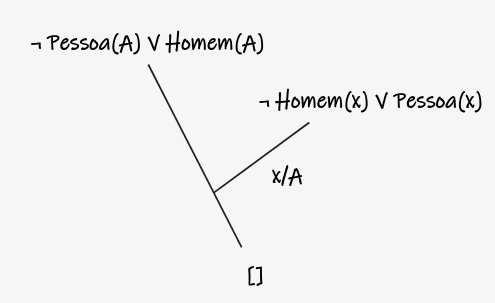
\includegraphics[width=7cm]{img/2_1.png}
% \end{figure}

\textbf{3)} Axioma:

$$PaiDeMedico \sqsubseteq \exists temFilho(Homem \sqcup Mulher) \sqcap \forall temFilho(Medico)$$

$$\forall x (t_x (PaiDeMedico) \rightarrow t_x(\exists temFilho(Homem \sqcup Mulher) \sqcap \forall temFilho(Medico)))$$

$$\forall x (PaiDeMedico(x) \rightarrow t_x(\exists temFilho(Homem \sqcup Mulher)) \land t_x (\forall temFilho(Medico))))$$

$$\forall x (PaiDeMedico(x) \rightarrow (\exists y (temFilho(x,y) \land t_y(Homem \sqcup Mulher))) \land (\forall y (temFilho(x,y) \rightarrow t_y(Medico))))$$

$$\forall x (PaiDeMedico(x) \rightarrow (\exists y (temFilho(x,y) \land (Homem(y) \lor Mulher(y)))) \land (\forall y (temFilho(x,y) \rightarrow Medico(y)))))$$

\textbf{4)} Conceitos:

$$Vegano \equiv Homem \sqcap \forall come.Planta$$
$$Vegetariano \equiv (Homem \sqcup Mulher) \sqcap \forall come.(Planta \sqcup Laticinio)$$
Vamos mostrar que $Vegano \sqsubseteq Vegetariano$ por \textbf{tableaux}%, ou seja, que $\forall x (Vegano(x) \rightarrow Vegetariano(x))$ e, por consequência, $\forall x (\neg Vegano(x) \lor Vegetariano(x))$
%$\forall Vegano \rightarrow Vegetariano)$ e, por consequência, $\forall x (\neg Vegano(x) \lor Vegetariano(x))$

\begin{itemize}
    \item [] $Vegano \sqcap \neg Vegetariano$ (x)
    \item [] $Vegano$ (x) \texttt{[**]}
    \item [] $Homem \sqcap \forall come.Planta$ (x) \texttt{[**]}
    \item [] $\neg Vegetariano$ (x) \texttt{[*]}
    \item [] $(\neg Homem \sqcap \neg Mulher) \sqcup \exists come.(\neg Planta \sqcap \neg Laticinio)$ (x) \texttt{[*]}
\end{itemize}

Primeira parte de \texttt{[*]}:

\begin{itemize}
    \item [] $\neg Homem \sqcap \neg Mulher$ (x)
    \item [] $\neg Mulher$ (x)
    \item [] $\neg Homem$ (x)
    \item [] $Homem$ (x) \texttt{[**]}
\end{itemize}

Segunda parte de \texttt{[*]}

\begin{itemize}
    \item [] $\exists come.(\neg Planta \sqcap \neg Laticinio))$ (x)
    \item [] $\exists come.(\neg Planta) \sqcap \exists come.(\neg Laticinio))$ (x)
    \item [] $\exists come.(\neg Planta)$ (x)
    \item [] $\forall come.Planta$ (x) \texttt{[**]}
\end{itemize}

Então, $Vegano \sqsubseteq Vegetariano$

% $$Vegano \sqcap \neg Vegetariano (x)$$
% $$Vegano(x)$$
% $$\neg Vegetariano (x)$$
% $$(\neg Homem \sqcap \neg Mulher) \sqcup \exists come.(\neg Planta \sqcap \neg Laticinio)(x,y)$$

% Segunda parte:

% $$\exists come.(\neg Planta \sqcap \neg Laticinio)(x,y)$$

% $$Homem \sqcap \forall come.Planta (x)$$ 
% $$ \neg Vegetariano (x)$$
% $$Homem (y)$$
% $$\forall come.Planta (x,y)$$
% $$\neg Vegetariano (x)$$
% $$ \neg ((Homem \sqcup Mulher) \sqcap \forall come.(Planta \sqcup Laticinio)) (x)$$
% $$ (\neg Homem \sqcap \neg Mulher) \sqcup \exists come.(\neg Planta \sqcap \neg Laticinio)) (x)$$

% % 

% $$\neg Homem \sqcap \neg Mulher$$
% $$\neg Homem$$
% $$\neg Mulher$$

% Segunda parte:

% $$\exists come.(\neg Planta \sqcap \neg Laticinio))$$



\end{document}